%qqqqqqqqqqqqqqqqqqqqqqqqqqqqqqqqqqqqqqqqqqqqqqqqqqqqqqqqqqqqqqqqqqqqqqqqq
%Quote
\begin{savequote}[50mm]
"
Supuestamente el cerebro humano es algo parecido a una libreta que se adquiere en la papelería: muy poco mecanismo y muchas hojas en blanco"\qauthor{Alan Turing}
\end{savequote}
%qqqqqqqqqqqqqqqqqqqqqqqqqqqqqqqqqqqqqqqqqqqqqqqqqqqqqqqqqqqqqqqqqqqqqqqqq

%*****************************************************

\chapter{Algoritmo y modelación}
\label{cha: Algoritmo y modelacion}
%*****************************************************
%El desarrollo de modelos computacionales permiten reproducir sucesos que escapan a acontecer de una vida humana. Es por eso la importancia de los modelos

En la búsqueda de poder conocer sobre el alineamiento de los SMBH en AGNs con su entorno, se hace necesario el uso de modelos computacionales que sean capaces de reproducir lo fenómenos físicos que ocurren en el Universo a gran escala y en los AGNs. Para nuestro propósito se hace uso de una serie de simulaciones cosmológicas auto-consistentes, que son capaces de simular la evolución de los espines de los SMBHs, su rata de acreción y el feadback producido,  entre otras propiedades de las galaxias. Las simulaciones se realizaron usaron el código Magneto-hidrodinámico para N-cuerpos AREPO \cite{springel2010}, que hace uso de mallas\footnote{Las mallas hace referencia a una driscretiación del espacio, que da como resultado una cuadrícula.} adaptativas, 
%capaz de reproducir mallas\footnote{Las mallas hace referencia a una driscretiación del espacio, que da como resultado una cuadrícula.} que cambian de forma y se mueven con el fluido a medida que corre la simulación,  
haciendo seguimiento a las propiedades del gas. Sin embargo, también se hace uso de otros métodos computacionales que permiten conocer cómo se distribuye la materia en el universo y mejor aun, permiten hacer una clasificación y estructuración. El método usado para la clasificación de estructuras en el universo es el  T-Web \cite{hahn2007}, capaz de clasificar las regiones del Universo usando un modelo de sistemas dinámicos. Para el modelo de detección de sub estructuras se hace uso del código Arepo, que emplea el método de subfind \cite{springel2018}, este permite localizar zonas de sobre densidad, identificando la presencia de halos de materia oscura, grupos y cúmulos de galaxias. 

%*****************************************************
\section{Código Arepo}
\label{sec: codigo arepo}
%***********************************************

%El código {\textsc{Arepo}} es una simulación cosmológica, que pretende diseñar una nueva forma de hacer simulaciones hidrodinámicas que son capaces reproducir la dinámica del universo, evolución estelar, formación de estructuras y evolución de parámetros en las galaxia. Este modelo hidrodinámico tiene como objetivo mejorar dos códigos muy usados en la simulaciones de formación y evolución: Mallado de Euleriano y la técnica  hidrodinámica de suavizado de partículas Lagrangiana (SPH). 

En la astrofísica se hace necesario poder contrastar los modelos teóricos con las observaciones. Por eso se emplea los modelos computacionales que parten de  modelos teóricos y buscan poder reproducir los resultados observacionales. En búsqueda de poder reproducir los procesos que ocurren en el universo, se considera la dinámica de fluidos, y con ello los modelos hidrodinámicos. Los modelos más sobresalientes en este ámbito son: hidrodinámica de la partícula suavizada (SPH) \cite{monaghan1992} e hidrodinámica Euleriana basada en mallas \cite{stone2008} con refinamiento adaptativo de las mallas (AMR). A pesar de ser los modelos más usados en la hidrodinámica presentan una serie de falencias:

- SPH ofrecen precisión de bajo orden para el tratamiento de discontinuidades de contacto, y en algunos casos suprime inestabilidades de los fluidos.

- Mallas Eulerianas no producen invariantes galileanos, implicando que los resultados son sensibles a grandes cambios en velocidades del fluido.\\

{\it{Arepo}} toma lo mejor de cada método hidrodinámico y mejora sus falencias. En general el código {\it{Arepo}} introduce una nueva forma de modelación hidrodinámica continua de mallas dinámicas \cite{springel2010}:

La precisión del código viene determinada mayormente por su forma de diseñar las mallas (grid). Se define la malla bajo la teselación de Voronoi de un conjunto de puntos que se distribuyen espacialmente.

El método de Voronoi es el método de interpolación más simple, que se basa en la distancia euclidea. Permite crear celdas de tal forma que la región encerrada por esta es lo más cerca posible a sus celdas vecinas. Los polígonos se diseñan al unir los puntos entre si, trazando luego una mediatriz entre los segmentos de unión. La intersección de las mediatrices dan como resultado los polígonos y por lo tanto la malla (ver figura \ref{fig: voronoi}). Cada celda en la malla lleva consigo variables de fluido que se conservan (masa, momentum y energía total).
%
\begin{center}
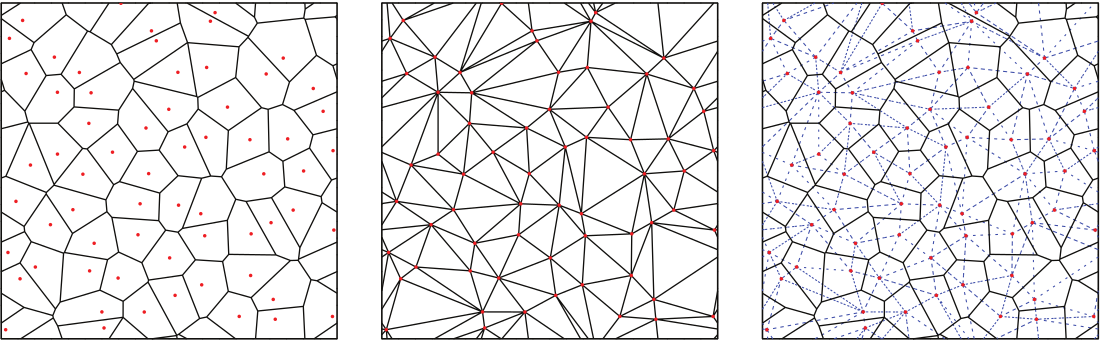
\includegraphics[scale=.35]{./figures/5_Algoritmo_Modelacion/voronoi.png}
\figcaption{\emph{Representación gráfica de la teselación de Voronoi y Delaunay. En esta gráfica se puede ver la doble topología del digrama de Voronoi, pues es equivalente topológicamente a la teselación de Delaunay. El panel al lado izquierda representa la teselación de Voronoi, el panel del centro a la teselación de Delaunay y el panel del lado derecho es la superposición de las dos teselaciones (linea punteada es teselación Delaunay y linea continua teselación de Voronoi). }}\label{fig: voronoi}
\end{center}
%
La importancia de usar el método de Voronoi en simulaciones  es que permite que los puntos en la malla se muevan con el fluido a la velocidad del fluido, esto garantiza que a medida que trascurren los pasos numéricos se actualice la información del fluido en la celda. Este método posibilita solucionar el problema de no invariabilidad galileana que emergía del método de la malla de Euler. Al solucionar esto se impide la alta sensibilidad en el cambio de las velocidades, haciendo que la dinámica del sistema sea consistente, y por ende se obtengan valores no sesgados para  el espín de los BHs y su disco de acreción.  

Este método permite que en las regiones donde hay una mayor sobre densidad de materia, se genere una mayor cantidad de celdas, proporcionando una modelación más precisa. Dando como resultado una mejor respuesta a la dinámica del fluido.
%aca voy
El objetivo principal de la simulación es poder solucionar las ecuaciones del fluido de manera muy precisa, para ello hace uso de las ecuaciones de Euler, que son leyes de la conservación de la masa, energía y momentum, que toma la forma de un sistema de ecuaciones diferenciales parciales hiperbólicas. \cite{springel2010} reescribe de forma compacta las ecuaciones de conservación del fluido de la siguiente forma:

Se introduce el vector de estado    
\begin{align}
    \vec{\bf{U}}= \begin{pmatrix} \rho \\ \rho\vec{v} \\ \rho e \end{pmatrix} = 
    \begin{pmatrix} \rho \\ \rho\vec{v} \\ \rho u+\frac{1}{2}\rho\vec{v}^{2} \end{pmatrix}\,,
\end{align}
donde $\rho$ es la densidad del fluido, $\vec{v}$ es el campo de velocidad y $e=u+ \vec{v}^{2}/2$ es la energía por unidad de masa. el parámetro $u$ indica la energía térmica por unidad de masa. Las cantidades del fluido son dependientes del espacio y del tiempo $\vec{\bf{U}}(\vec{\bf{x}},t)$, se define además la función de flujo

\begin{align}
    \vec{\bf{F}}(\vec{\bf{U}})=
    \begin{pmatrix} \rho\vec{v} \\ \rho\vec{v}\vec{v}^{T}+ P \\ (\rho e + P)\vec{v} \end{pmatrix}\,,
\end{align}
donde $P$ es la presión del fluido. Por tanto  la ecuación de Euler se puede escribir de forma compacta como 
\begin{align}
    \frac{\partial\vec{\bf{U}}}{\partial t} + \vec{\nabla}\cdot \vec{\bf{F}}\,.
\end{align}

En el código {\it{Arepo}} se considera una discretización del fluido cómo un conjunto de volúmenes finitos, donde cada celda se identifica bajo el uso de un contador "$i$". Cada celda contiene la información de la masa $m_{i}$, momentum $p_{i}$ y la energía $E_{i}$. %
\begin{align}
    {\bf{Q}_{i}} = \begin{pmatrix} m_{i} \\ p_{i} \\ E_{i} \end{pmatrix} = \int_{V_{i}} \vec{\bf{U}}d\vec{\bf{V}}\,.
\end{align}
%
Usando la ecuación de Euler, es posible calcular la razón de cambio de ${\bf{Q}_{i}}$ en el tiempo, al usar el teorema de Gauss
%\
\begin{align}
    \frac{d{\bf{Q_{i}}}}{dt} = -\int_{\partial V_{i}}[\vec{\bf{F}}(\vec{\bf{U}})-\vec{\bf{U}}\vec{\bf{w}}^{T}]d\vec{\bf{n}}\,,
\end{align}
donde $\vec{\bf{w}}$ es la velocidad de cada partícula y $\vec{\bf{n}}$ es el vector normal a la superficie.

El esquema presentado por \cite{springel2010} indica cuales son los pasos (algoritmia) que sigue el código. Parte del vector de estado del fluido para cada celda ${\bf{Q_{i}}}$ y al hacerlo evolucionar es capaz de dar los resultados de no invarianza galileana y buena resolución. 

%*****************************************************
\section{Caracterización del entorno}
\label{sec: Caracterizacion entorno}
%*****************************************************

Al recordar lo mencionado en la sección (\ref{sec: Estructure_Formation}), es posible decir que las simulaciones computacionales, 
%asumiendo el régimen lineal o no lineal, 
son capaces de reproducir la estructura del Universo, donde estructura hace referencia a una organización u ordenamiento de la materia, a causa del potencial gravitacional. Las sobre densidades en el Universo permiten encontrar y caracterizar los diferentes tipos de estructuras.
%Al obtener la estructura del universo se observa la emergencia de regiones donde hay un cambio en la densidades (una abundancia de materia), donde la estructura cambia considerablemente.

%----------------------------------------------------    
    \subsection{Método T-Web}
    \label{subsec: Metodo_T-web}
%----------------------------------------------------
Al considerar el método propuesto por \cite{hahn2007} es posible argumentar lo siguiente: Asumiendo la teoría concerniente a los sistemas dinámicos, se realiza un análisis de estabilidad local para orbitas de prueba en cada celda que resulta de la discretización del volumen de la simulación, y alrededor de halos de materia oscura. Donde cada una de las partículas de prueba se mueven por acción de un potencial gravitacional $\phi$.

La ecuación de movimiento que describe la trayectoria de la partícula en coordenadas comóviles está dada por 
\begin{align}
    \ddot{x}=-\nabla\phi\,.
\end{align}
%
Al asumir que el potencial gravitacional $\phi$ está actuando en el centro de masa ($\bar{x}_{i}$) produciendo un máximo local,  da como resultado lo siguiente:
%
\begin{align}
    \nabla\phi(\bar{x}_{i})=0\,.
\end{align}
%
Con esto es posible linealizar la ecuación de movimiento en los puntos donde es máximo ($\bar{x}_{i}$)
%
\begin{align}
    \ddot{x}_{i}=-T_{ij}({\bf{\bar{x}}_{k}})(x_{j}-\bar{x}_{k,j})\,,
\end{align}
%
donde $T_{ij}$ es el tensor de marea dado por el Hessiano del potencial gravitacional
%
\begin{align}
    T_{ij}=\frac{\partial^2 \phi}{\partial r_{i} \partial r_{j}}\,.
\end{align}
%
Este tensor de marea puede ser representado por una matriz real simétrica 3x3, con autovalores $\lambda_{1}>\lambda_{2}>\lambda_{3}$ y  autovectores $\vec{e}_{1},\, \vec{e}_{2},\, \vec{e}_{3}$. Los autovalores son de gran importancia a la hora de clasificar el entorno cosmológico, estos son los indicadores de la estabilidad de la orbita de las partículas de prueba, que se mueven en la dirección del autovector \cite{padmanabhan1995}, \cite{hahn2007}.

Al usar la teoría de \cite{zeldovich1970}, que se estudió en la sección (\ref{subsubsec:Zeldovich_Aproximation}), es posible definir una clasificación a partir de los autovalores en cada región del espacio:\\

$i)$ {\it{Vacíos (voids)}: Región del espacio donde los tres autovalores $\lambda$ son negativos (orbita estable), indicando una divergencia o expansión en esa región.}\\

$ii)$ {\it{Hoja (sheet)}: Región donde hay un autovalor positivo $\lambda_{1}>0$ y dos negativos $\lambda_{2} \leq \lambda_{3}< 0$, esto indica un colapso en una dirección del espacio mientras que en las otras dos hay una expansión.}\\

$iii)$ {\it{Filamentos (filament)}: Región del espacio donde solo hay un autovalor negativo $\lambda_{3}\leq 0$, indicando que hay un colapso en dos direcciones y expansión en una.} \\

$iv)$ {\it{Nudo (knot, cluster)}: Región donde los tres autovalores son positivos, dando como resultado un colapso en las tres direcciones, formando una región de convergencia.}\\

En la figura (\ref{fig: formacion de estructura con autovalores}), es posible observar los cuatro casos donde se representan los tipos de estructuras dependiendo del autovalor.
%
\begin{center}
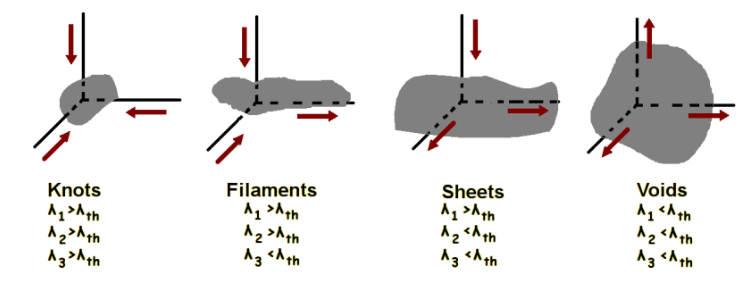
\includegraphics[scale=.39]{./figures/5_Algoritmo_Modelacion/formacion_estructuras.png}
\figcaption{\emph{El valor de los autovalores permiten clasificar el tipo de estructura en la cual se encuentran \cite{bustamente01}.}}\label{fig: formacion de estructura con autovalores}
\end{center}
%
Lo destacable de este método es su análisis meramente dinámico, lo cual le da más importancia que los métodos que usan principios meramente geométricos, permitiendo identificar zonas de igual densidad pero con propiedades dinámicas de estabilidad diferente. La desventaja de este procedimiento es su dependencia de los máximos locales (hablando del campo de densidad). 
Ya que estos máximos solo son posibles al interior de los halos de materia oscura, implica un problema en la resolución y precisión en el método, ya que no se analiza todas las regiones del espacio. Para
dar solución a este problema se aplica un suavizado gaussiano a los máximo encontrados.
%reducir la aparición de máximos locales inexistentes resultado de la falta de resolución, se aplica un suavizado gaussiano.
%La desventaja de este procedimiento es que depende altamente de los mínimos locales, que solo son justificados en el interior de halos de materia oscura, careciendo de resolución y precisión para lugares diferente a los halos.


El código que se esta implementando para la clasificación del entorno, hace uso del valor "límite" $\lambda_{th}$ para la clasificación \cite{bustamante2015}, pasando de ser $\lambda_{th}=0$ a $\lambda_{th}=0.265$. Se hace uso de este valor límite, porque es capaz de trazar de muy buena forma la red cósmica. 

\begin{figure} 
\centering 
\subfloat{
%\label{fig: función de masa estelar}
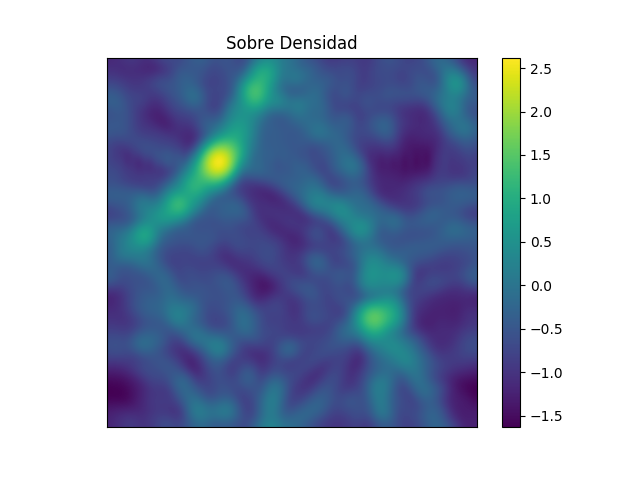
\includegraphics[width=0.43\textwidth]{./figures/5_Algoritmo_Modelacion/Distribution_density_inferior.png}} 
\subfloat{ 
%\label{fig: función de masa BHs}
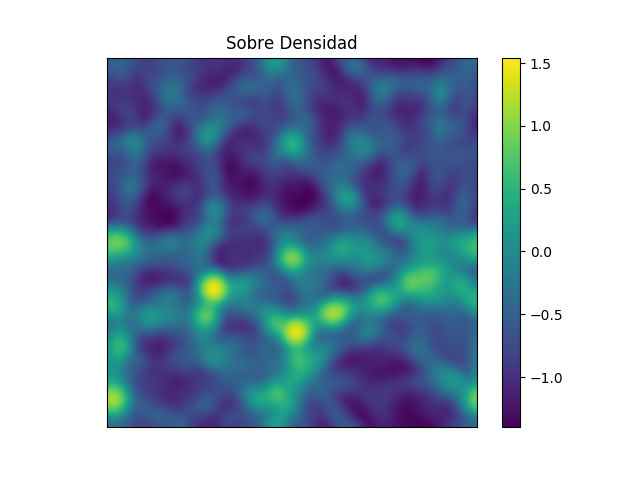
\includegraphics[width=0.43\textwidth]{./figures/5_Algoritmo_Modelacion/Distribution_density_media.png}} 
\subfloat{ 
%\label{fig: función de masa halos}
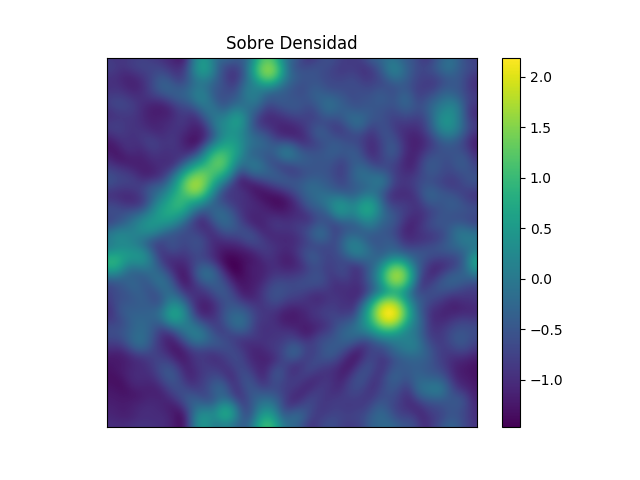
\includegraphics[width=0.43\textwidth]{./figures/5_Algoritmo_Modelacion/Distribution_density_superior.png}}
\caption{\emph{Distribución del campo de sobre densidad, resultado del modelo T-Web, las figuras son cortes en el eje $z$ a diferentes alturas. La figura superior izquierda representa un corte inferior, la superior derecha un corte medio  y la inferior da cuenta del corte superior.}} 
\label{fig: Campo de densidad } 
\end{figure}




%*****************************************************
\section{Método de detección de subestructuras}
\label{sec: detección sub-estructuras}
%*****************************************************

Una vez se obtiene la clasificación del entorno a gran escala (red cósmica), es necesario poder conocer cómo se distribuye la materia en el interior de estas estructuras, por esto se hace necesario un criterio para clasificación de sub-estructuras. La continuidad de la distribución de materia en el universo implica un  problema a la hora de caracterizar la materia en dichas sub-estructuras. Poder discretizar la distribución de materia en el espacio posibilita hacer uso de modelos computacionales, capaces de identificar las estructuras internas.

%----------------------------------------------------    
    \subsection{Método de FoF}
    \label{subsec: FoF}
%----------------------------------------------------

Es uno de los métodos más usados para la detección de estructuras en simulaciones cosmológicas, FoF proviene de las siglas {\it{friend of friend}}, debido a la comparación entre vecinos o ``amigos". Es usado en gran medida para la comparación de modelos computacionales de la distribución de materia en el Universo.
%,  determinando que tan confiable es el modelo contrastado. 

El método FoF se basa en 
encontrar intercepciones entre volúmenes definidos alrededor de partículas (ver figura  \ref{fig: FoF esquema}).  
%La región dada por el volumen $4/3\pi R_{i}^{3}$ es llamada región de vinculación. 
La región de vinculación se define como esferas de radio $R_{i}$ concéntricas a la partícula, dada por la expresión \cite{bustamente01}:
%
\begin{align}
    R_{i}=b\ell\,,
\end{align}
%
donde b es el parámetro de vinculación y $\ell$ es la distancia promedio entre las partículas.

Este método consiste en ubicarse en cada partícula y calcular su región de vinculación, posteriormente calcular la región de vinculación de las partículas vecina o amigas, con esto se determinan las intercepciones y posibilita la identificación de la estructura.
Estas estructuras serán caracterizadas por la cantidad y ubicación de las partículas vinculadas. 
%
\begin{center}
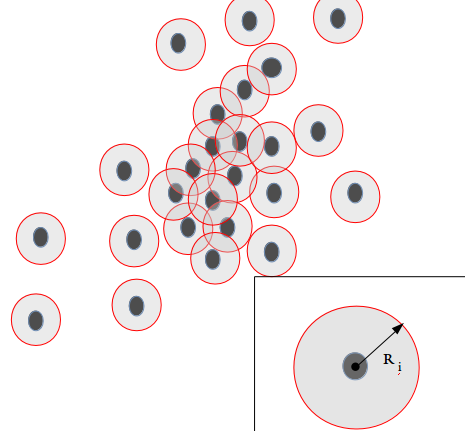
\includegraphics[scale=.35]{./figures/5_Algoritmo_Modelacion/FoF_metodo.png}
\figcaption{\emph{Esquema de cómo funciona el método de FoF, consiste en determinar que partículas interactuan entre sí a partir de la intersección de regiones de vinculación. }}\label{fig: FoF esquema}
\end{center}
%

%----------------------------------------------------    
    \subsection{Algoritmo Subfind}
    \label{subsec: Algoritmo subfind}
%----------------------------------------------------

Subfind es un método computacional usado para extraer de forma refinada las sub-estructuras en simulaciones cosmológicas. Esta herramienta es más precisa que FoF pero presenta un costo computacional mayor, sin embargo el uso de los dos método permiten optimizar la clasificación de las estructuras. El primer paso que realiza el método {\it{subfind}} es calcular las densidades de las posiciones para todas las partículas en un grupo. Esto se realiza usando SPH, con una escala de suavizado a una distancia del $n$ vecino más cercano, y la densidad es calculada por la interpolación del núcleo sobre sus vecinos. Se considera cualquier región que presente una sobre densidad para ser una candidata a subestructura, e.i. se define una región contenida o encerrada por un contorno de isodensidad que traspasa un punto de silla. Para obtener estas regiones se parte de algún núcleo local de sobre densidad, se desplaza alrededor del núcleo de forma concéntrica evaluando la sobre densidad, a medida que se aleja del centro el umbral global de densidad va disminuyendo, una vez haya un aumento en este umbral  se indicando una intersección con otra región de sobre densidad. El lugar donde ocurre la intersección permite definir el contorno de dicha sobre densidad. Es necesario tener en cuenta que los contornos entre dos regiones se unen en un punto de silla, dando como resultado un cambio en la topología de contorno de la isodensidad.

La importancia de este método es que permite clasificar de forma  refinada una gran variedad de subestructura, que dan como resultado una lista de candidatos a subhalos. Para una mejor descripción de este método se recomienda \cite{springel2018}.

La mejor forma de optimizar el proceso de determinación de estructuras y subestructuras, es encontrar el máximo de densidad con el método de FoF y a partir de allí usar {\it{subfind}} para determinar las sub-estructuras alrededor de este núcleo.

%es allí donde se define una región de dicha sobre densidad. 

%a partir de ello determina las regiones de sobre densidad (abundancias de materia), en estas sobre densidades se ubican los máximos locales se desplaza hacia el exterior del máximo de forma constante. Cuando se encuentre un aumento en la sobre densidad, este aumento de densidad indica la presencia de una sobre densidad  

%una vez  obtiene estas regiones de sobre densidad se procede a construir esferoides concéntricos al lugar donde ocurre la sobre densidad. Cuando la densidad de la región albergada dentro del esferoide es equivalente a aproximadamente 200 veces la densidad media del universo, que en otras palabras es equivalente al equilibrio virial, se detiene la construcción de esferoides y determina una sub-estructura \cite{springel2018}.















%***********************************************************************